%!TEX root = ../../thesis.tex
\section{Synthesizer}
\label{impl-synth}

\begin{lstlisting}[language=JavaScript, caption=A synthesizer's data structure, label=lst:synth]
{
  "position": 1,
  "synthSettings": Object,
  "tones": [{
    "position": 0,
    "duration": 1,
    "note": "A2",
    "id": "tone_22"
  }]
}
\end{lstlisting}

The data structure of a synthesizer is the largest of all pieces because it contains the settings for each individual parameter of each synthesizer module (see \reffigure{fig:editor-concept-synth-settings}). All these settings are however omitted in \reflisting{lst:synth} because they would take up too much space. The \code{synthSettings} property (line 4) is basically a key-value description of the parameters. Each tone that should be played by the synthesizer is listed in the \code{tones} array. They consist of a \code{position} property (line 5), which describes the relative position of the tone in the current piece, a \code{duration}  property (line 6), which describes how long a tone is played, and the \code{note} property (line 7) which defines the pitch of the current note.

\medskip
\begin{figure}[htb]
  \centerline{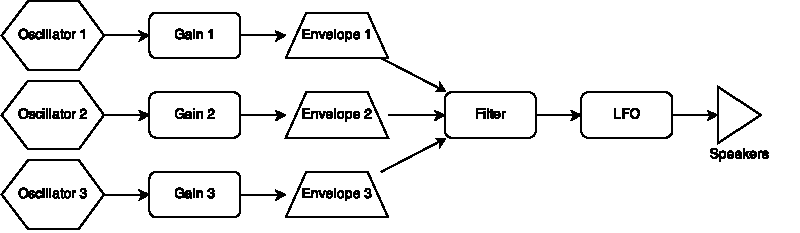
\includegraphics[width=\linewidth]{images/SynthesizerNodeGraph.pdf}}
  \caption[The synthesizer's node graph]{The synthesizer's node graph}
  \label{fig:synth-node-graph}
\end{figure}

The synthesizer that has been implemented for this editor is based on the early Moog synthesizer's design and its node graph is shown in \reffigure{fig:synth-node-graph}. It is a polyphonic synthesizer that uses three oscillators to generate the base sound. Each oscillator is routed through its own gain node which influences the volume of this specific oscillator and therefore it influences its impact in the mixed signal in the end. The gain node passes the signal on to an envelope which influences the oscillator's volume over time and from there it is passed to the filter. The filter shapes the sound of the mixed signal and passes it on to the Low Frequency Modulator which then influences the volume in an alternating manner. The LFO then passes the signal on to the speakers.

All modules haven been built from the base nodes which are supported by the Web Audio API and the envelope is based on the envelope which has already been sketched out in \refchapter{sec:adsr-envelope}. In order to play a tone, the tone's \code{note} property needs to be transferred into a base frequency which will then be the frequency that is used for each oscillator. The implementation of this translation is based on Stuart Memo's algorithm from his `QWERTY hancock' library\footnote{\url{http://stuartmemo.com/qwerty-hancock/}, last checked on 17/03/2014}.

One big challenge in implementing the synthesizer was that a manual garbage collection of unneeded oscillator nodes was needed because the amount of oscillator nodes grew fast over time and unused oscillators have a huge performance impact on the overall application. The algorithm for the garbage collection runs during the playback of the synthesizer piece and checks for unused and finished nodes at a specific interval which is based on a pre-calculated overall amount of needed nodes and the time that is between the tones.

The note grid's implementation, which was already shown in \refchapter{concept-synth-grid}, is based on the drag and drop elements that were already used in other pieces like the recording piece (see \refchapter{impl-recording-piece}). One tone in the grid consists of two draggable nodes. One that influences the relative position of the tone and one that influences the width, and therefore the duration, of the tone.